% !TEX root = ../../thesis.tex

\cleartoleftpage
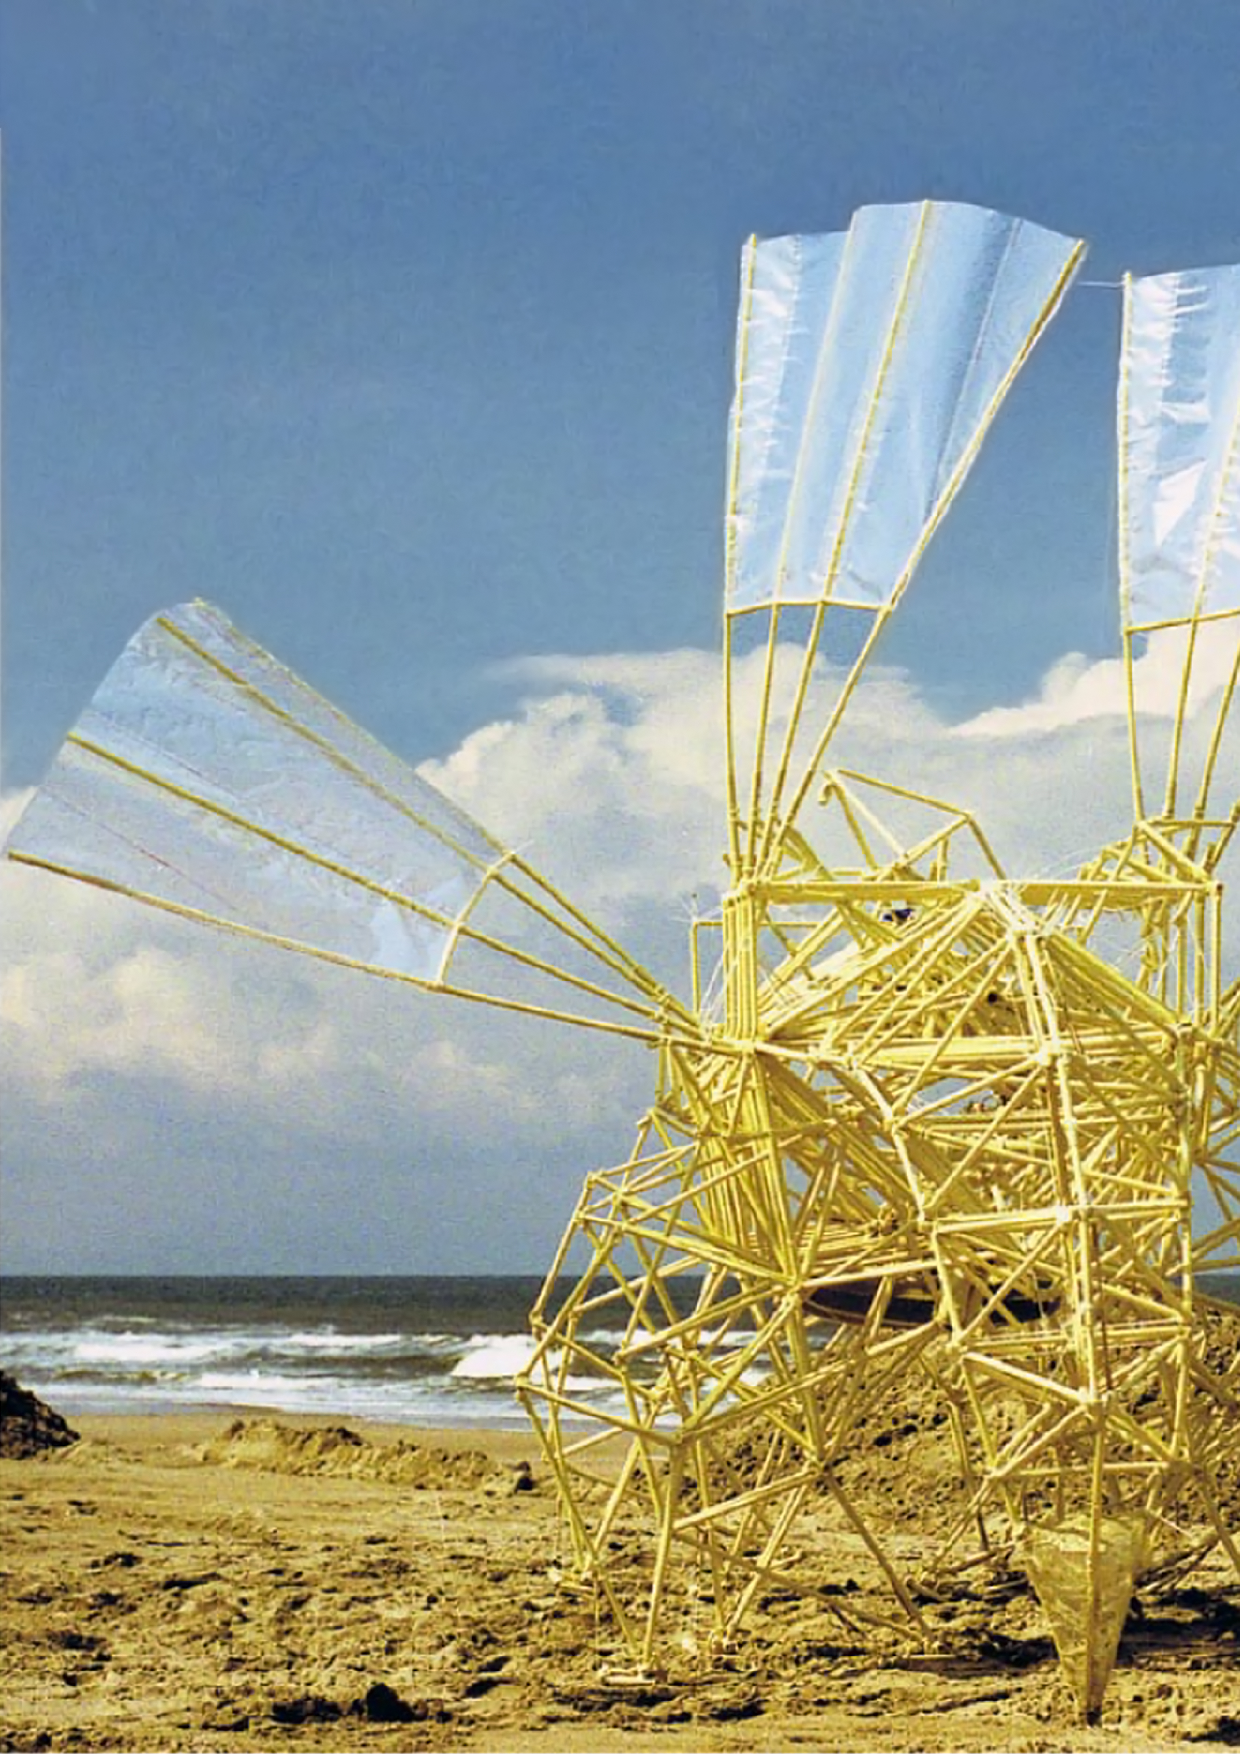
\includepdf{../media/chapter_illustration/jansen.pdf}

% Kant les hommes sont comme les oiseaux

\chapter{Robot morphology: some fascinating work} % (fold)

\cleanchapterquote{The cognition needs a body to think}{Rodney Brooks}

\section{The cognitivist approach limits} % (fold)

In 1949, the Elmer and Elsie robots, also known as turtle robots (see \figurename~\ref{fig:walter_robot}), created by the cybernetic pioneer W. Grey Walter, can be considered as one of the first robots in the robotics modern history era (1950-now). Back at this time, the transistor was just invented (1948)~\cite{brinkman1997history} and calculus was done with mechanical machines (see the focusbox). The turtle robot was entirely analogical but was able to demonstrate complex behaviors (see \figurename~\ref{fig:turtle_behavior}). Without any "reflexion" or internal representation of itself and the world, this robot, thanks to its conception and the direct analogical interaction between sensors and actuators was able to avoid obstacles and reach its charing station~\cite{walter1950imitation}. These complex behaviors which can be compared with ones found in nature were in fact done without any kind of intelligence and were actually emergent from interaction between the robot morphology (i.e. where are placed sensors and how they are connected with actuator) and the robot environment (i.e. light sources).

\begin{figure}[]
\centering
    \subfloat[][]{\label{fig:walter_robot}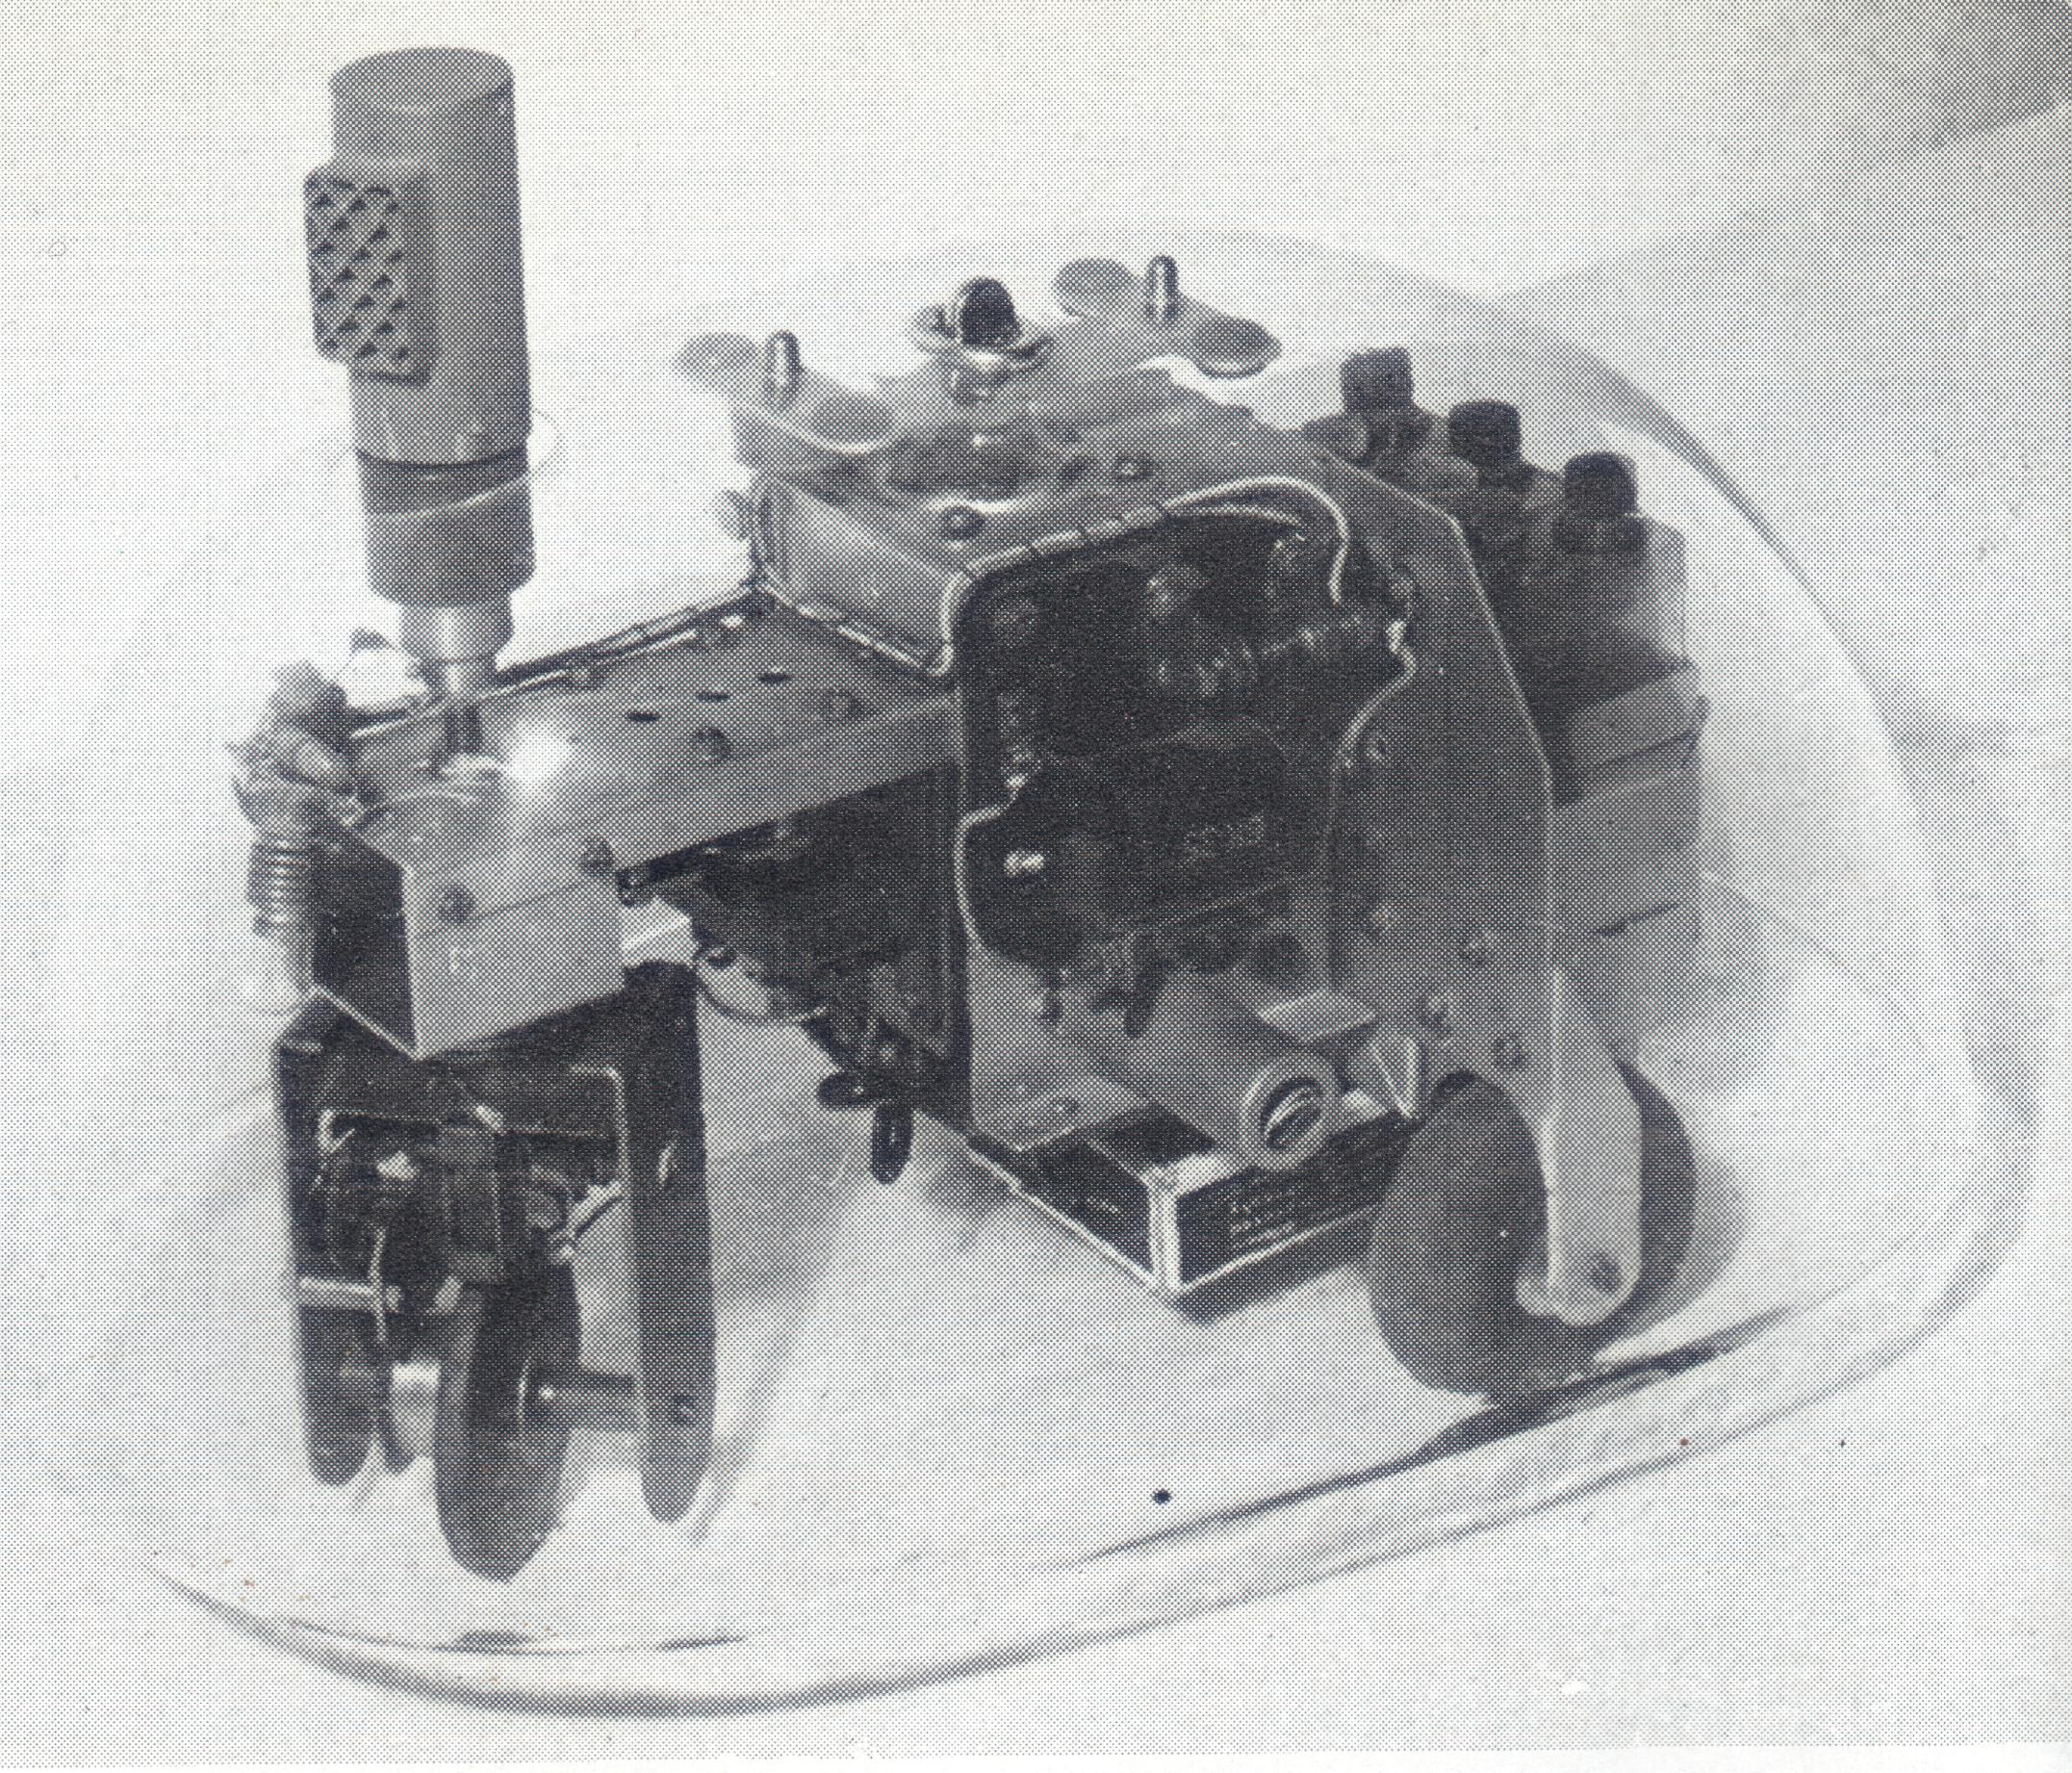
\includegraphics[height=6.5cm]{walter_turtoise_robot.jpg}}
    \hfil
    \subfloat[][]{\label{fig:turtle_behavior}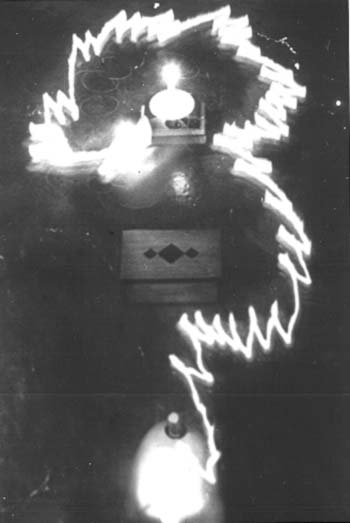
\includegraphics[height=6.5cm]{turtoise_behavior.jpg}}
    \caption{}
    \label{fig:turtle_robot}
\end{figure}

\begin{figure}[]
    \centering
    \begin{boxedminipage}{0.95\textwidth}
        \textbf{Mechanical calculus}\\
        Once upon a time, in a age transistors were not here, complex calculus was done using mechanical properties.
        Using complex mechanisms the very first calculators were fully mechanical machine (see \figurename~\ref{fig:mechanical_computer}).

        The first freely programmable, binary, floating-point, general-purpose mechanical computer in the world was the Z1 constructed by Zuse between 1936 and 1938 (see \figurename~\ref{fig:zuse_z1}).
        This "computer" contained approximately 30,000 components and was incredibly sophisticated, making the Z1 suitable for a wide variety of engineering and scientific applications.
        Introduced by Curt Herzstark in 1948, the Curta (see \figurename~\ref{fig:curta_calculator}) is a small, hand-cranked digital mechanical calculator.
        It can be used to perform addition, subtraction, multiplication, division, and (with more difficulty) square roots and other operations.
        The Curta's design is a descendant of Gottfried Leibniz's Stepped Reckoner and Thomas's Arithmometer, accumulating values on cogs, which are added or complemented by a stepped drum mechanism.
        It has an extremely compact design: a small cylinder that fits in the palm of the hand.

        These two examples show that even pure calculus is achievable using only morphological properties (here mechanical) and was used during dozens of years for scientific applications.


        Curtas were considered the best portable calculators available until they were displaced by electronic calculators in the 1970s.

        \begin{center}

            \subfloat[][Zuse Z1 (1936)]{\label{fig:zuse_z1}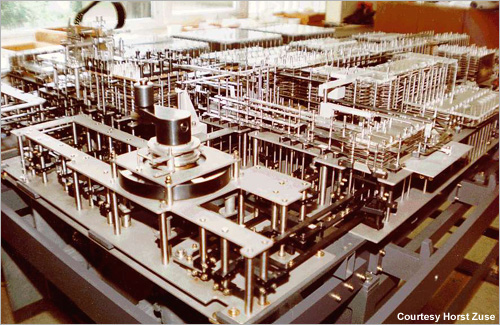
\includegraphics[width=0.42\linewidth]{hist-z1-reconstruct.jpg}}
            \hfil
            \subfloat[][Curta]{\label{fig:curta_calculator}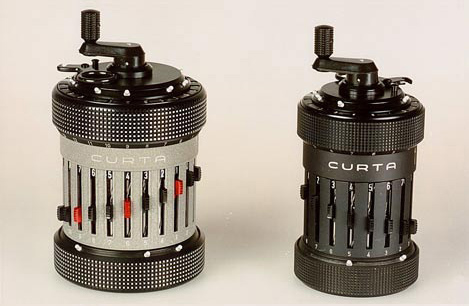
\includegraphics[width=0.42\linewidth]{curta_calculator.jpg}}
            \caption{Mechanical calculus machines}
            \label{fig:mechanical_computer}

        \end{center}

    \end{boxedminipage}
\end{figure}

With the arrival of numeric computers, researchers imagined the opening of a field where it could be possible to replace pre-wired analogical electronic behaviors by the use of computer running programs. Not dependent on the hardware platform, robots would be therefore more versatile.
The artificial intelligence (AI) term was introduced in a workshop organized in 1956 by a MIT professor John McCarthy (REF). Globally participant were convinced, that by using the notion of computation or abstract symbol manipulation, it would be possible to reproduce interesting abilities similar to human ones~\cite{kaufmann1979machines}~\cite{haugeland1989artificial}. The symbol-processing paradigm or cognitivistic paradigm see the cognition as pure computation. In other word, the actual intelligence process is the abstract algorithm or the program doing calculus. Eventually, researchers following this paradigm no longer saw the physical incarnation as a relevant component. Cognitive and computationalists hypotheses stating that the thought is reducible to a set of symbolic calculations are being established~\cite{fodor1987psychosemantics}. The body, for its part, is forgotten, irreparably separated from the mechanisms of intelligence~\cite{kaplan2008corps}.
In addition, the robot body became a handicap which often ruins the efficiency of algorithms and programs created by AI researchers. Indeed, the real world body is non perfect, there is some noise on sensors acquisition, there is gravity, friction and inertia acting on actuators, and the environment is always changing and unpredictable.

To overcome these issues of real world applications, the other side of the robotics community, still interested in the hardware challenges strives to design more reliable and powerful robots which can react as fast and as close as possible to the model used for its control. To do that, it is needed to have way more precise sensors and powerful enough actuators to overcome inertia and mechanical friction. Thanks to these work on hardware, industrial robots became more and more fast and precise, enough to outclass any human on specific assembly tasks.

However, even with really efficient robots, artificial intelligence failed to show results comparable with the expectations researchers and society had. Robots are able to solve incredibly complex task such as chess game or able to achieve highly precise tasks in manufacture but require perfectly controlled and predictable environment. Going outside this known environment seems impossible to program and none of them is able to act fluently in the real world.

Thus classical approach known great successes to solve abstract problems such as chess game, search engine, text processing, however it failed in the understanding of natural forms of intelligence which requires a direct interaction with the real world. This is especially the case when we think in the current state of the art for interaction with human (natural language) or object (grasping) and the locomotion in an open environment (walk, run, ride a bicycle).


\section{The emergence of embodiment paradigm} % (fold)

Stuck with these major issues raised by acting in the real world, a kind of crisis of the artificial intelligence happened in the 1980's and the cognitivist paradigm was questioned. While some researchers of the field introduced new tools such as neuronal networks, another part questioned the "cognition is computation" approach and the irrelevance of the body.
Thanks to researchers such as Rodney Brooks~\cite{brooks1986achieving}, Rolf Pfeifer~\cite{pfeifer2001understanding} or Luc Steels~\cite{steels1995artificial}, a novel paradigm emerge: the cognition needs a body to think. The embodied artificial intelligence rejects the symbolic approach and postulates that it is not possible to have intelligence without the body and the environment~\cite{pfeifer2001understanding}. Rather than postulating there is a hierarchical structure in which the brain control the body, the new theory focuses on the interaction between the two systems, even for mathematical thinking we could assume is purely abstract~\cite{lakoff2000mathematics}.

Following this paradigm, several researchers tried to tackle challenges in which the classical cognitivist approach failed i.e. the understanding of natural forms of intelligence which requires a direct interaction with the real world. The locomotion is a great example of task where the classical robotic approaches did not get expected results.

Animals are incredibly skilled. Even if we consider insect with a brain thousand of times smaller than the human one, theirs abilities to move in an open world is just incomparable with the most advanced current robots. One important reasons for this is that in the classical view, the ability to figure out where you are is based in detailed inner models or representations either have to be programmed into the robots or learn by interacting with the environment and continuously updated. The more complex these models are, the more effort is needed to acquire the relevant data to maintain them leading to major problem when learning task in a highly dimensional spaces (plein de REF). Brooks even argued that intelligence always requires a body and that we should forget about complex internal representations and models of the outside world; that we should not focus on sophisticated reasoning processes but rather capitalizer on the system-environment interaction~\cite{brooks1991intelligence}~\cite{brooks1995intelligence}. Then he started to work on the insect locomotion because if we understand the insect-level-intelligence it will be much easier and faster to understand and build human-level intelligence~\cite{brooks1996prospects}.

\textbf{TODO: petite review du boulot de brooks avec les insects}

Exploring the role of the morphology and how it shapes the ways we think appears a fascinating open field. Indeed, exploring the interaction between body properties and cognition could lead to both a better understanding of animal's behaviors (human being in particular) and to build robot more adapted and robust to an open environment with unpredictable interaction.

Thus an interesting evolution of the last decades is the demonstration of the importance of the morphology for sensorimotor control, cognition and development. The researches community exploring the embodiment paradigm has grown but surprisingly not as much we could imagine with classical paradigm fails. However, new work arises introducing new principles we will describe in this chapter such as morphological computation, compliance or ecological balance, emergence.

In the context of this thesis we will talk about intelligence with the meaning, ability to move in a natural environment and interact with people and objects.


% \begin{figure}[]
%     \centering
%     \begin{boxedminipage}{0.95\textwidth}

%         \textbf{Planes fly only thanks to their morphologies}\\

%         One of the major engineering achievement of the Twenty-th century has been the understanding of the fly and the realization of efficient plane both for commercial and military application.

%         A priori there

%         If we study a complex behavior such as the ability to fly. Using a cognitivist paradigm, the fly would require a large amount of explicit calculus.  With this approach we could think the fly need a large amount of explicit calculus. However the aeronautic people already understand that the plan they are trying to make fly will act in the real world and the real world is the "air". A plane can only fly because of the air and because it is viscous. The air is not a constraints it is the central element for make a plane fly.

%         Indeed a plane has to deal with its environnement which is the "air".

%         % While ones could see the real air as a constraint because of its viscousness and prefer model it as a perfect fluid in simulation, it would be impossible or at least way more complicated to make a plane fly. Indeed, it is because the air is viscous that the fly is possible.

%         Actually a plane fly only thanks to the interaction between its specific wing morphology and the environnment fluid which is the "air".

%         \begin{equation}
%             F_{lift} = \frac12 \times \rho \times V^2\times S \times C_z
%         \end{equation}

%         To create lift, the only variable are the profil shape which give the $C_z$ parameter and the surface voilure $S$ and the air properties with its volumic mass $\rho$ and the velocity of the flux $V$.

%         \begin{equation}
%             adapted morphology + air = fly
%         \end{equation}


%         All the intelliegence is centered around the wing shape.


%         % Another great example of how mechanics properties can produce complex behavior is the airplane.
%         % The lift force generated by wings are the resulting of the interaction between a air flux and the physical profil shape of the wing.
%         % Then the Bernouilli law add the necessary magic around to make plane fly (see \figurename~\ref{fig:magic_plane})

%         we can change the behavior by changing the wing shape, some fighters have a voilure variable

%         Forme des ailes etc ...

%         To resume, a plane can work thanks to the fact the air is not a perfect fluid and because it has an adapted morphology. Even rocket use aerodynamic to improve the stability otherwise it would be really complex to keep a direction.



%         % The only way to make machine "fly" without these specificities is to create a rocket which need a very high power to oppose the gravity and complex control to

%         % \begin{figure}[tb]
%         %     \begin{center}
%         %         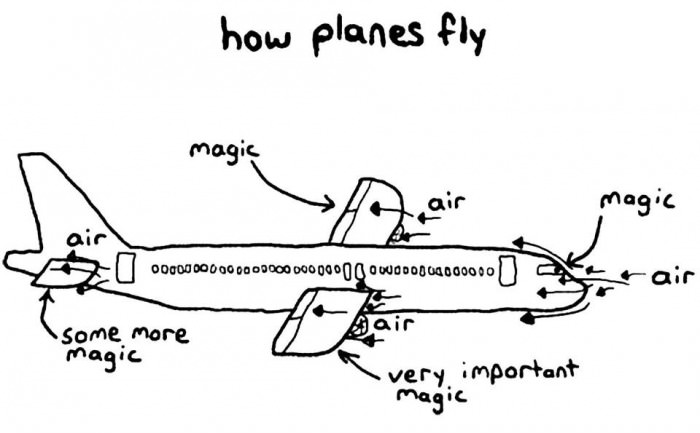
\includegraphics[width=0.8\linewidth]{plane_explanation.jpg}
%         %     \end{center}
%         %     \caption{Caption here}
%         %     \label{fig:magic_plane}
%         % \end{figure}

%         \begin{center}[]
%         \centering
%             \subfloat[][]{\label{}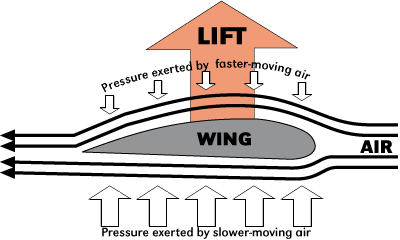
\includegraphics[width=0.4\linewidth]{bernoulli_wing_lift.png}}
%             \hfil
%             \subfloat[][]{\label{}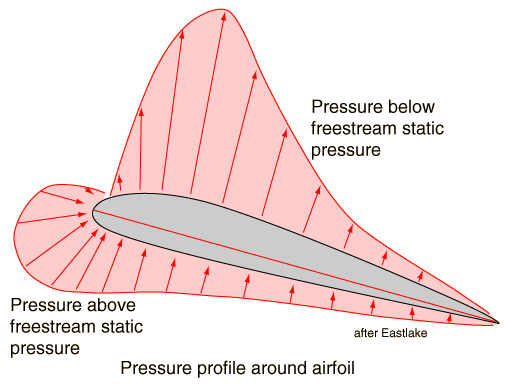
\includegraphics[width=0.3\linewidth]{airfoil_bernouilli.png}}
%             \caption{}
%             \label{fig:}
%         \end{center}

%         After 60 years of fly history with hundreds of actual plane from planneur to airbus A380, it looks obvious that the shape of the plane is a major, or event the most important part. However, then discussing of legged locomotion, from centipedes to biped ones, the question of the morphology is often left aside in favor to computationnal model. Is there really a fundamental reason the body should be irrelevant for legged locomotion while being essential for flying? There is a lot of legged animals and they are not smater than the flying or swimming ones. Is there a fundamental law comparable to the Bernouilli one ? It can be a biological, a mechanical or even a chimical law, yet it deserves to be explored.

%         While the velocity of legged locomotion are in most of the case quite low, we could ignore air friction, then a first track could be the interaction between the newton's law and the ground. Using gravity as an advantage instead of a force we have to battle.

%     \end{boxedminipage}
% \end{figure}


\section{Morphological computation} % (fold)

As we saw in the introduction, with the arrival of numeric computing, the interest for the robot body seemed less and less relevant for artificial intelligence researchers. They used the "think is calculate" paradigm, a cognitivist approach which globally failed in the understanding of natural forms of intelligence which requires a direct interaction with the real world.
However, while we can think there are indeed calculus necessary to achieve complex tasks, there is no reason it should be explicit with a precise internal model or representation of the physical world. Then it could be directly done by through body properties.

Following the definition of the robotic morphology given by C.Paul:
\begin{quotation}
The morphology of a robot thus refers to the physical structure and form of a robot. Specifically, the focus is on characteristics such as link sizes, number of links, joint characteristics, mass distribution, actuator characteristics, material properties, sensor characteristics and sensor placements. In short, any characteristic which defines the physical structure of the robot is included in the term morphology.
\signed{Chandana Paul~\cite{paul2006morphological}}
\end{quotation}

The morphological computation principle states that a part of the computation needed in the achievement of a given task can be done implicitly through the interaction of physical form with the ecological niche environment.

We are particularly interested in this thesis in the role of morphology for the locomotion and interaction in the human ecological niche.

For decades and it is still mostly the case, the challenge of locomotion for robotic agent was only tackles through symbolic abstract and complex computation of internal model and representation of the world. However, regarding the nature, it appears obvious that an animal morphology deeply change the way it can act in its ecological system and so it has evolved trying to optimize its body properties.

For some reasons, in the robotics and artificial intelligence field the link between the body properties and the ability for a robot to move in an ecological environment does not seems as obvious. The fact that the ability to do thing is due to the brain computation is so deeply grounded than it affects even the general public.

Since the 80's, the fact that the morphology of a robot affects its control requirements has become increasingly evident in robotics. Not only does the morphology determine the behaviors that can be performed, but also the amount of control required for these behaviors. Particularly in systems where behavior is obtained through purely sensory-motor interactions of the body with the environment, the morphology is of prime importance. Nonetheless, even in other robotic systems, a relationship has been found to exist between morphology and control requirements, in that some morphologies yield themselves to being more easily controlled than others.

This relationship was first observed and characterized by Pfeifer as the morphology and control trade-off ~\cite{pfeifer2001understanding}, but the mechanisms underlying this relationship have been unclear. The fact that simple physical interactions give rise to computation indicates the theoretical possibility for the dynamics of the morphology to play a computational role in the system, and thereby to subsume part of the role of control~\cite{paulinvestigation}

However, beyond the animal kingdom evidence, the human being already understood this principle in other domains. As in this thesis we are more concerned about the locomotion, we can cite all the vehicules allowing human to locomote in various way invented. Most of the vehicule we used today were invented before the apparition of computer science and were totaly functionnal without any kind of explicit computationnal intelligence.

A car, for example, is an autonomous system able to move in wide range of environnement from perfect asphalt circuit to deep jungle mainly thanks to the damper it has. There is no computaiton of the correct wheel position given a model of the external world and a planning path. The position is just due to the interaction of the car damper properties and the ground.

Another great example is the plane. Make a machine fly is one of the great scientific and engeenering example acheived thanks to a deep understanding of the interaction between the environnement and the morphology.



\subsection{Passive and Semi-Passive Walkers} % (fold)

Tad McGeer


This set-up the work of Tad McGeer, comming from the aeronautic field, he was surprised by how the actual legged robot morphology was neglected. A great example is the Tad McGeer's passive walker. Thanks to the understanding of the intrinsic dynamics of its structure, Tad McGeer has managed to create a 2D biped robot capable of producing several steps without any controller or motor showing that such a complex task can be indeed achieved only with adapted morphology\cite{mcgeer1990passive}.

The result is comparable to the sailplane or the paper plane. Using a specific mass repartition and foot shape interecting with gravity and the ground ...

The role of morphology in robot biped locomotion has been particularly explored through the research on passive dynamic walkers~\cite{wisse2007passive}.
The most famous example concerns the Tad MacGeer's work~\cite{mcgeer1990passive}.
Thanks to the understanding of the intrinsic dynamics of its structure, McGeer has managed to create a 2D biped robot capable of producing several steps without any controller or motor.
The only control of this robot is obtained through the interaction between the intrinsic inertia of the structure and gravity.

\begin{figure}[]
\centering
    \subfloat[][Tad McGeer with his prototypes]{\label{fig:tad_mcgeer}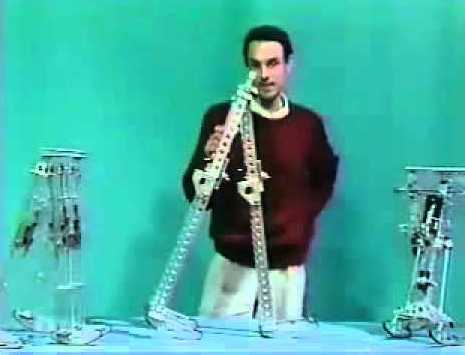
\includegraphics[width=0.49\linewidth]{tad_mcgeer.jpg}}
    \hfil
    \subfloat[][Passive walker robot]{\label{fig:mcgeer_walker}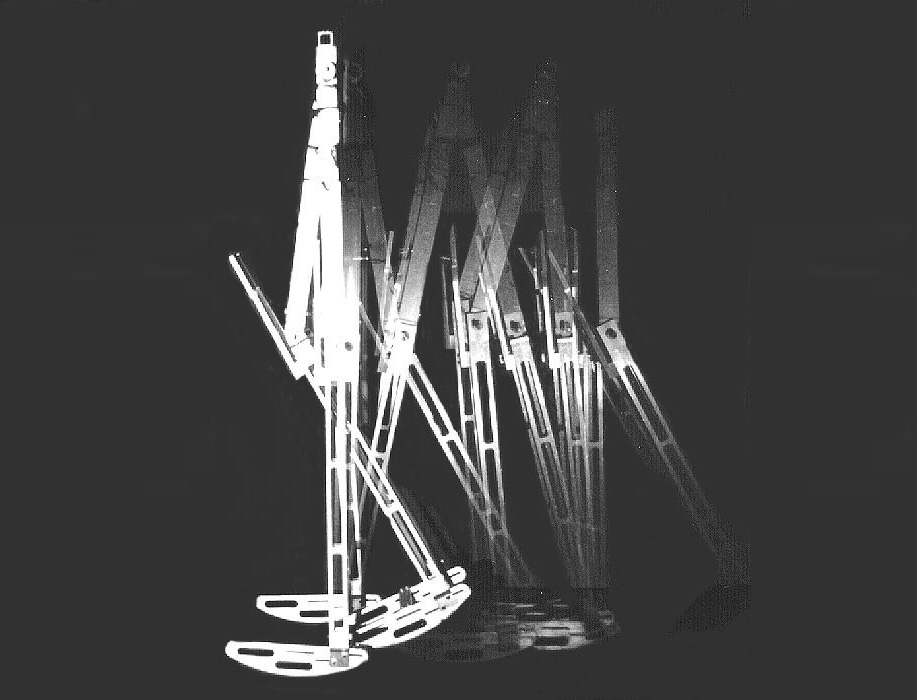
\includegraphics[width=0.49\linewidth]{mcgeer_walker.jpg}}
    \caption{}
    \label{fig:mcgeer_work}
\end{figure}

This work has been pursued with the apparition of semi-passive walker combining both specific passive properties and low power actuation to increase their robustness~\cite{Anderson2005}.
We can note the work of Collins~\cite{collins2005bipedal} which explored the case of semi-passive 3D biped robot.
Its morphology is based on particular mass distribution, knee locking, round feet and springs on the legs to generate an efficient walking gait while keeping its lateral and frontal balance.
The concept of 3D semi-passive robot has been pushed even further with the realization of a complete humanoid robot with trunk, arms and head: the robot Denise~\cite{wisse2005three} and Flame presented in~\cite{Hobbelen2008}.

http://tensegritywiki.blogspot.fr/2010/08/mechanism-as-mind-tensegrity-and.html

we could make a parrallel the energy consumed to th
\begin{figure}[]
    \begin{center}
        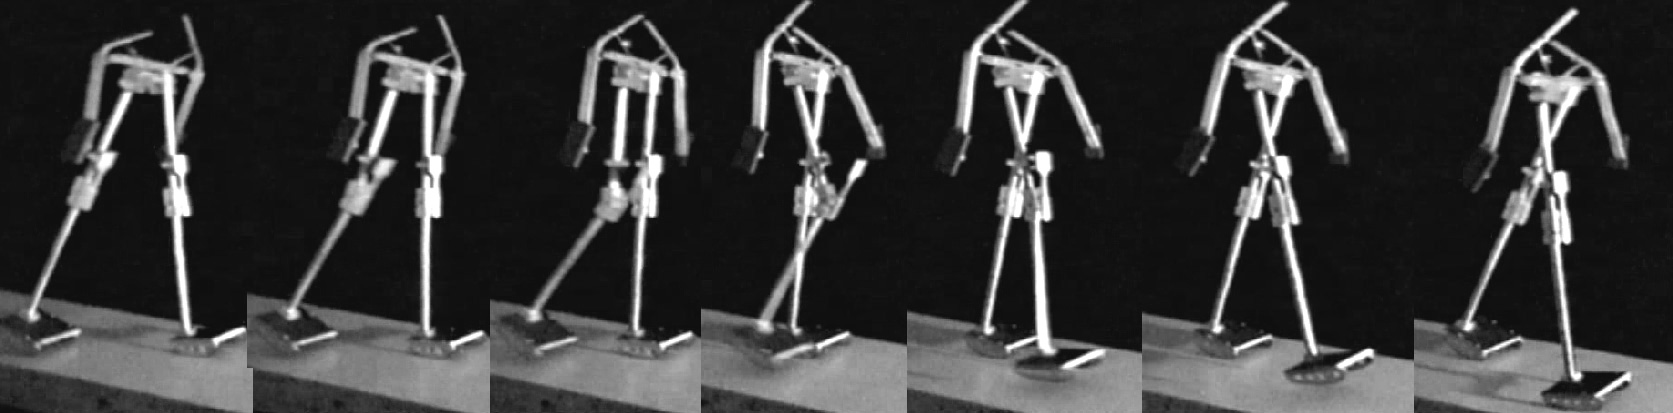
\includegraphics[width=0.99\linewidth]{cornell_biped_series.jpg}
    \end{center}
    \caption{Caption here}
    \label{fig:figure1}
\end{figure}

\begin{figure}[]
    \begin{center}
        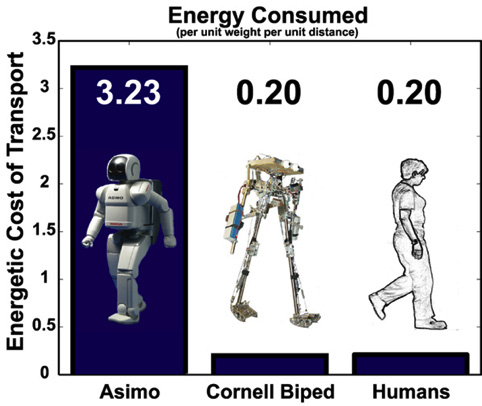
\includegraphics[width=0.6\linewidth]{comparison_cost_transport.jpg}
    \end{center}
    \caption{Caption here}
    \label{fig:figure1}
\end{figure}

\subsection{humans} % (fold)
\label{sub:humans}

% subsection humans (end)
It has also been shown that human morphological properties such as the compliance of the body explains the dynamics of walking and running \cite{Geyer2006} while experiments made by Kojiro Matsushita~\cite{matsushita2005locomoting} show that an adequate morphology is needed if one is interested in natural looking kind of locomotion.


\section{The compliant and soft robotics} % (fold)
It has also been shown that the compliance of the body explains the dynamics of walking and running \cite{Geyer2006} and several biped robots such as Athlete Robot \cite{niiyama2010athlete} or BioBiped1 \cite{radkhah2011concept} were designed using compliant actuator or elastic material.

\section{Ecological balance}

The concept of morphological computation has also been associated to the principle of “ecological balance”, as outlined by Pfeifer et al.\cite{pfeifer2005new}, which states that there is a balance or task distribution between morphology, materials, control, and interaction with the environment.

\section{Emergence of complex behavior} % (fold)

\subsection{The sandbeast} % (fold)

We should not only interest ourself
Some very interesting proofs of concept can be found in the complen

In Art, complementary work can be found. It is the case of The Jansen genius artist. Outside the research community, we can find


\begin{figure}[]
    \begin{center}
        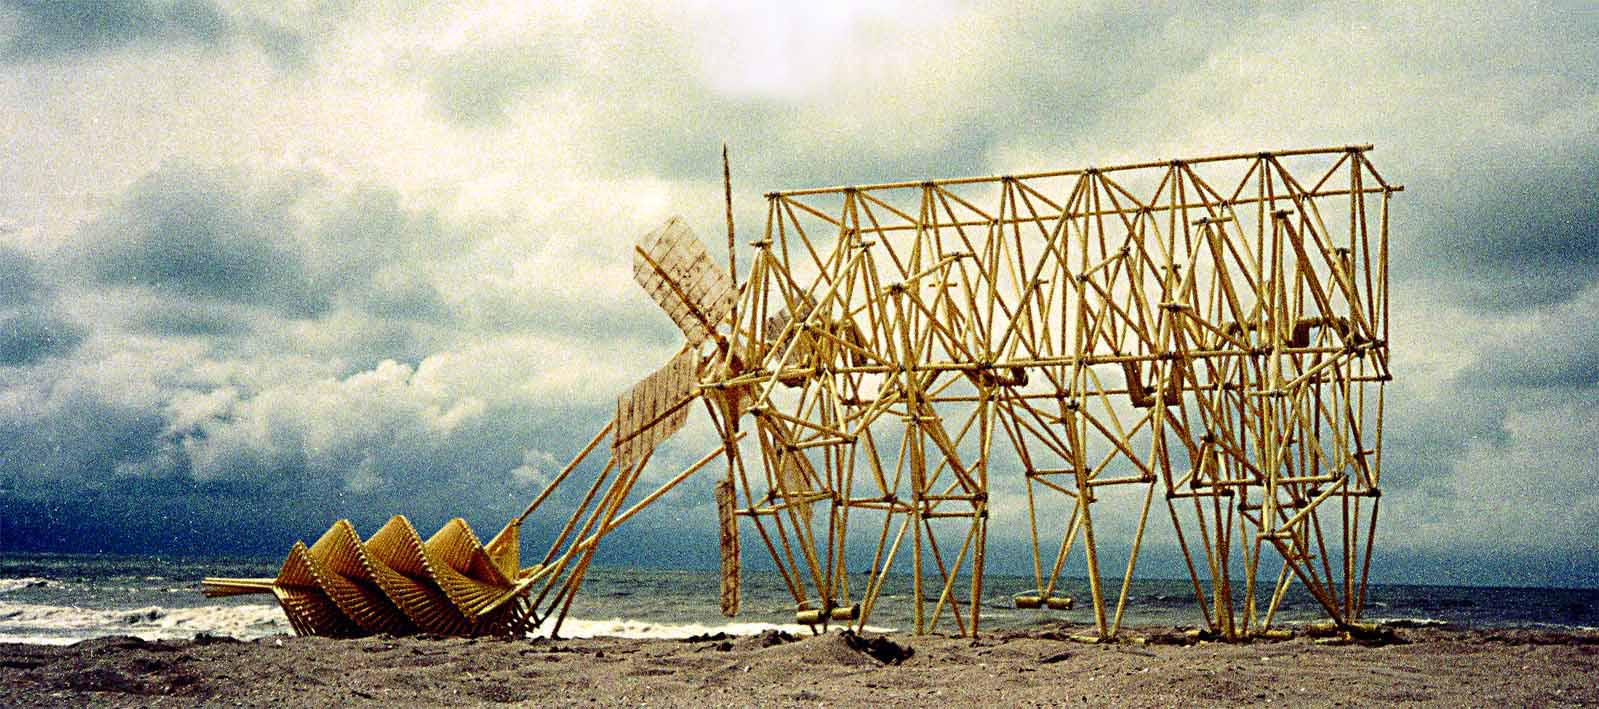
\includegraphics[width=0.99\linewidth]{theo_jansen_beast.jpg}
    \end{center}
    \caption{Caption here}
    \label{fig:theo_jansen_beast}
\end{figure}

Theo Jansen is a sculptor in the kinematic art field. This artist playing with field frontiers, between engineering, research and art is the designer of the sand beasts (see \figurename~\ref{fig:theo_jansen_beast}).
These giant structure move using a really clever mechanisms composed of eleven rods which lenghts have benn tuned through optimization. This system produces a walking motion(see \figurename~\ref{fig:beast_mechanism}) with the center always remaining at the same level, for this reason Theo Jansen likes to say he "reinvented the wheel" but adapted to the environmental niche of his creatures, the beach.

During the XX years of this work, Theo Jansen created dozens of creatures, more and more evolved. However, the very basic mechanism remains the same, both simple because it is composed by only one degree of freedom, and complex because the length ratio between links are critical and must be equal to specific numbers The Janson called gold or god numbers.

Thus, using only really basic material, electric plastic tubes, Theo Jansen created multi-legged creatures capable of moving in the sand, powered by the wind.


\begin{figure}[]
\centering
    \subfloat[][]{\label{}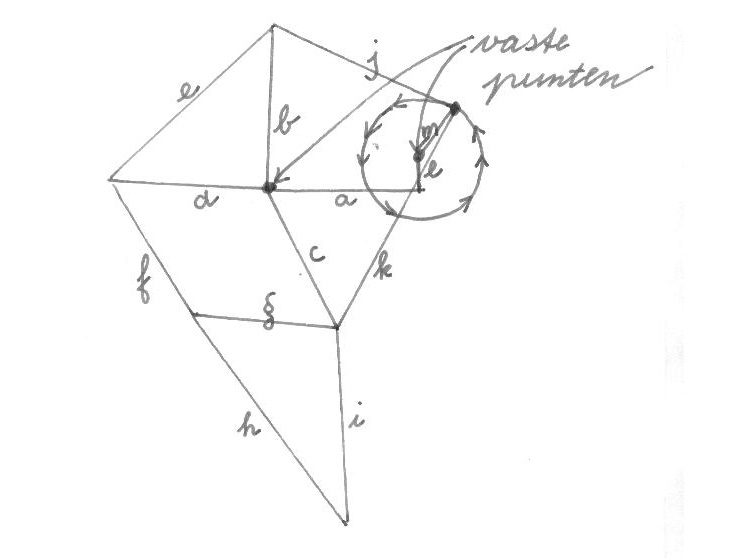
\includegraphics[width=0.32\linewidth]{strandbeest_theory.jpg}}
    \hfil
    \subfloat[][]{\label{}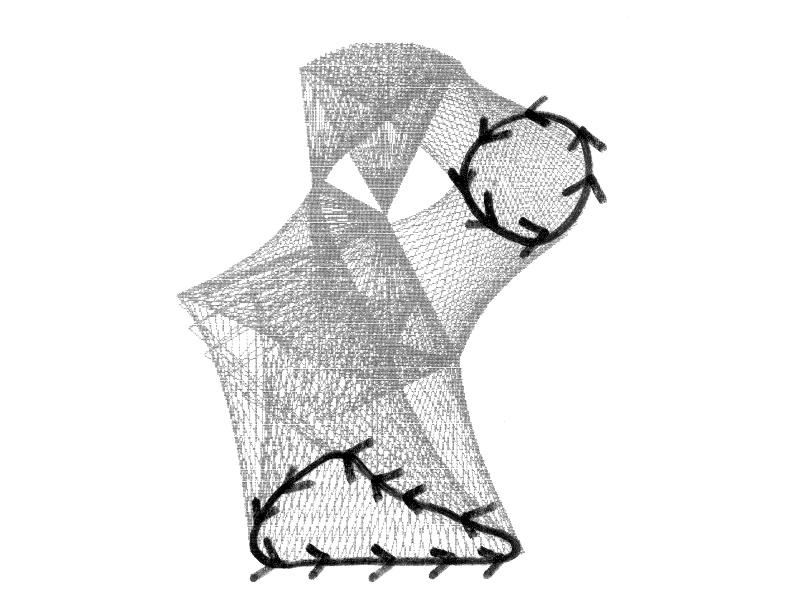
\includegraphics[width=0.32\linewidth]{strandbeest_motion.jpg}}
    \hfil
    \subfloat[][]{\label{}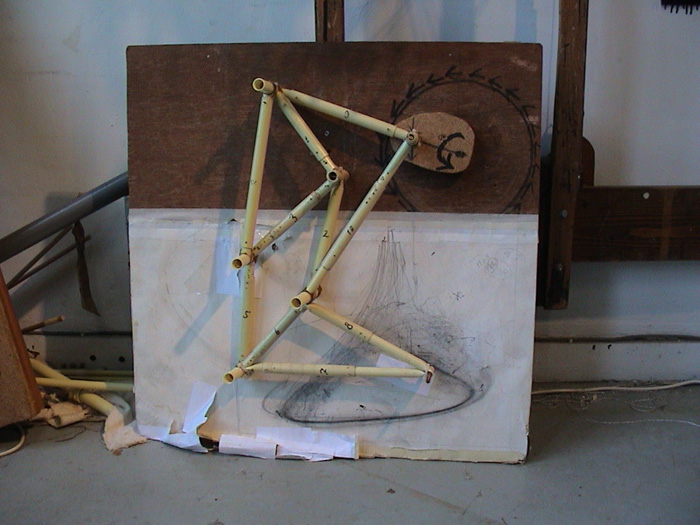
\includegraphics[width=0.32\linewidth]{strandbeest_leg_element.jpg}}
    \caption{}
    \label{fig:beast_mechanism}
\end{figure}



Evolution of his work, conducted to several improvements. For instance, he added lemonade bottle to store energy. These bottle are used as pressure tank fulled using pumps powered by the wind. Beasts can use this stored energy in case the wind fade away.

Also, a natural enemy of these beasts is the sea, using the same basic material, Theo Jansen created sensors able to detect the water and reverse the way beast move. The same principle allows also these beast to avoid obstacle.

Thus the work of Theo Jansen goes beyond the kinematic art and is really instructive for the robotic and IA research fields. Indeed, thanks to a specific morphology adapted to their environmental niche, his creatures are able to act autonomously and "survive" in the real world. No computation, no abstraction, the appeared intelligence of these creatures only came from a direct interaction between their particular morphologies and the environment. It is, for me, a meaningful proof of concept.

\url{https://www.youtube.com/watch?v=rWbU3eV4ZpQ}
72 legs moving at the same time using one cranks

\subsection{Acroban} % (fold)
\label{sub:acroban}
Among all robots designed to explore morphological computation and compliant body only few allow to explore physical interaction such as Kenshiro \cite{Asano2012} or Acroban which the compliant structure of its vertebral column and legs was shown to permit a self-organized physical human-robot interface allowing non-expert users to lead the robot by the hand \cite{Ly2011bio}\cite{Oudeyer2011}.
% subsection acroban (end)

\subsection{Ijspert} % (fold)
\label{sub:ijspert}

% subsection ijspert (end)
PARLER DE LA SALAMANDRE DE IJSPERT
For example, morphological computation has been shown to be necessary in order to achieve human-like biped locomotion \cite{matsushita2005locomoting} and the coupling of adequate morphologies with central-pattern generators has been shown to generate robust locomotor behavior \cite{ijspeert2007swimming}\cite{steingrube2010self}.








\section{Robotic} % (fold)
For years, artificial intelligence was only considered through complex computation.
An interesting evolution during the last decade was the emergence of work showing the importance of the actual robot morphology in the robot behavior.






These robots showed interesting hopping and running behavior while using less power actuator than common humanoid robot such as Asimo or HRP-2.



The morphological properties of these robotic platforms are especially interesting but unfortunately they are difficult and expensive to reproduce by other research laboratories.
Most of the studies made on the humanoid robot locomotion in the past 30 years~\cite{park1998biped}~\cite{aoi2005locomotion}~\cite{park1998biped} mainly focus on tackling the challenge of biped walking through the active control of the whole robot dynamics using technics such as ZMP control~\cite{vukobratovic2004zero} requiring very precise and high torque actuation~\cite{akachi2005development}.

The properties of the robot morphology have shown interesting results for robust locomotion, for instance the hexapod robot Rhex~\cite{saranli2001rhex}.
Still, it is surprising that only few explored the challenge of biped locomotion through the study of the role of morphology.
One can cite the work of Chandana Paul and Josh C.Bongard~\cite{paul2001road} and Ken Endo~\cite{endo2002co} which have explored evolutionary optimization on robot morphology to achieve stable biped locomotion.
They have showed a strong impact of the morphology on the walking behavior and were able to reduce the complexity of the controller by finding good mechanical properties (limbs length and mass distribution).


\section{Conclusion} % (fold)

Scientific study of the role of morphology in sensorimotor control and cognition: in Robotics (McGeer, Pfeifer and co.), in relation with Cognitive Science (e.g.
http://www.pyoudeyer.com/IEEETAMDOudeyer10.pdf ) and animals (e.g.
work of Robert Full)

EmbedIT – An Open Robotic Kit for Education
\url{http://www.eucognition.org/index.php?page=tutorials}




\section*{stuff}
Cognition from the bottom up: on biological inspiration, body morphology, and soft materials Rolf Pfeifer1, Fumiya Iida2, and Max Lungarella3

http://spectrum.ieee.org/automaton/robotics/robotics-hardware/fast-running-biped-robot-based-on-velociraptor

http://spectrum.ieee.org/automaton/robotics/robotics-hardware/japanese-quadruped-robot-pneupard

\section*{stuff to put inside from Pfeifer book}

p44. In the mid-90s, Brooks argued that we have now achieved the "insect level intelligence". Ghengis, Attila et Hannibal, three of Brooks six-legged robots have achieved impressive walking performance in terms of obstacle avoidance and walking over uneven ground. However, insects can do many more things such as navigation or manipulation.

Speak about the Cog project: development of humanoid robot with the goal of eventually reaching high-level cognition.

p45. The term humanoid robot is used for robots that typically have two arms and legs, a torso and a movable head with vision system and sometimes additional sensory modalities such as audio and touch. They are called humanoid because ther is a superficial visual resemblance to humans.

p45.Because of their anthropomorphic shape, people have a strong tendency to project humanlike properties onto these robots. David McFarland's reference to anthropomorphization as an incurable disease.


p55. The synthetic methodology states that by actually building physical agents -real robots- we can learn a lot about nature of intelligence. Physical agents by bringing together results from all the different areas have a highly integrative function. In addition, they allow for concrete testing of ideas in an objectif way: a robot either works or it does not.

p78.The synthetic methodology "understanding by building". We build a system that mimics certain aspects of the behavior we wish to study. This way of proceeding has proved enormously powerful: because you have to build somethong that actually works in the real world, there is no way of glossing over details, which is possible when you formulate a theory abstractly.
Grey Walter's turtles and Braintenberg's vehicules illustrate a very important and a t first quite surprising result: very simple brains, in the right context, can produce seemingly complex behavior that we might even want to call intelligent.


The boids flock on the basis of three simple local rules of interaction: collision avoidance, velocity matching or alignment, and flock centering. p220
The results of experience is amazing given the simplicity of the rules.

Given a certain desired behavior, devising the rules that will lead to the desired behavior is more difficult than explaining the behavior if the system is run i.e if the agent interacts with its environment. THis is called design of emergence (Steels 1991) and it is still an open questoin how this can be done systematically. At the moment, design for emergence is an art rather than a hard-core enginnering discipline. Because the fact that the behavior itself cannot be preprogramed but is always the result of an agent-environment interaction, we must design for emergence rather than directly for a specific behaior.
Evolutionary roboticist Inman harvey of the University of Sussex is right when he proclaims "design is out, evolution is in!". suite p87

Unlike virtual workds, the real-world challenges an agent in various ways. First, because real-world agents are emboied, acquisition of information always take time. Second information thatn an agent can acquire about real world is always very limited. We can never have complete information. This situation is different from a formal game like chess, where knowledge of the board positon constitutes all the information about the state of the game. Third information acquired trhough them will always contain errors. Fourth the real world s not characterized by clearly defined, discrete  states, the weather is never simply goof or bad.
The real wolrd has its own dynamics -things out in the world happen even if not do anything- ther is always time presure due to ongoing change. Thus agent are always forced to act whether they want to or not.
Related to this point, the real world is a highly complex dynamical system, making it intrinsically unpredictable because of its nonlinear nature and its sensivity to initial conditions (hebert Simon has coined the term bounded rationality to designate, in essence, decisions that have to be taken under such circumstances (Simon, 1976,1969e)).

